\label{Anexos}
\appendix
\clearpage
\addappheadtotoc
\appendixpage
\chapter[Anexo I: Fisc. Virtual/Inf. para elecciones en Neuquén]{Anexo I: Fiscalización Virtual/Informático para elecciones en Neuquén}
En Febrero de 2019 se participó como fiscales informáticos para Unidad Ciudadana en las elecciones provinciales de Neuquén para ese mismo año. La misión de un fiscal es verificar y auditar el sistema a utilizar en la emisión de sufragio, las boletas y el sistema de recuento provisorio. El objeto es detectar cualquier situación que pudiera poner en riesgo la transparencia o la equidad en los comicios, o llevar a confusión al elector. Para llevar adelante este proceso la Justicia Electoral de Neuquén convocó a diferentes agrupaciones políticas para auditar la quema de DVDs y la prueba de transmisión. Estos DVDs son el medio para iniciar y habilitar las máquinas para su posterior uso en la votación. La prueba de transmisión se ejecuta sobre una máquina que contiene los mismos componentes que las máquinas de votación pero utiliza otro software, esta máquina además se conecta a internet y ejecuta un sistema preparado para transmitir los datos de escrutinio. 

\section{Quema de DVDs el día 28/02/2019}
Se participó durante la audiencia para la quema de 2000 DVDs (1504 mesas + 500 de backup) utilizados para iniciar las máquinas del sistema de boleta única electrónica (BUE). \newline
Esta actividad se realizó en una sala dividida en dos secciones, una fue utilizada para los fiscales de diferentes partidos, y otra para personas de la justicia y la empresa.  \newline
El evento comienza con una explicación del proceso a realizar por parte de la Justicia Electoral.  La organización informa que existe un solo software utilizado para toda la elección. Cada autoridad de mesa contará con una tarjeta personal con un chip que permite activar las categorías disponibles para la mesa que corresponda. Es decir, en las localidades donde sólo se elige gobernador, el sistema muestra Gobernador-Diputados-Consejeros y en las ciudades donde también se elige intendente, se muestra además los Intendentes y Concejales de esa localidad. \newline
Luego se muestra un DVD (el master) cuyo contenido no es accesible, del cual solo se conoce que se utiliza el método de hash sha512sum da la firma: \newline
8d7b20cf8f3d101a3253ca7af1ae91c0d24cd36af3371ad65daa295f224f83a7e89d0ccbe21fabb2393c1b \newline 153118c369423b92de5a5a1204f0c84e5c7f2687d7  \newline
Se procede con la primera copia de 6 DVDs y se valida que coincida la firma con el DVD master.  
Se pone a disposición 3 máquinas (una de las cuales no inició y fue reemplazada) para probar el sistema. Se visualiza el sistema desde un punto de vista funcional, haciendo todo el proceso desde la apertura de la mesa hasta el cierre. En las pruebas hechas no hubo errores detectados. Se testearon tres disposiciones de candidatos (Neuquen Capital, Centenario y Chos Malal) por un periodo de 15 minutos. 
Al momento de responder consultas sobre el desarrollo del sistema, los referentes presentes en la exposición responden que no poseen conocimientos técnicos sobre el software utilizado. Además, se consulta sobre el sistema que se encarga de transferir los datos desde la escuela al centro de cómputos, respondiendo que la máquina utilizada para tal fin es la misma con la cual se realizan los votos, con la diferencia que el DVD utilizado es distinto y esta máquina se encuentra apartada de las demás conectada a la red de internet de la escuela. \newline
En resumen, este día se auditaron las copias que se realizaron verificando que posea el mismo hash que el master.  Del master se pudieron hacer algunas pruebas de funcionamiento correcta, pero no se permitió auditar el código fuente. Por lo tanto, no se pudo garantizar: 
 \begin{itemize}
     \item que la disposición de las opciones sea siempre aleatoria y que se presenten todos los candidatos 
     \item que imprima en la boleta lo seleccionado 
     \item que el contenido del chip sea igual a lo impreso en la boleta papel 
     \item que el proceso de conteo sea correcto 
     \item que se imprima el resultado final correcto 
     \item que el contenido del chip del acta de cierre sea igual a lo impreso en el acta papel 
     \item que los datos que se transfieren de la escuela sean iguales al acta papel
     \item la integridad de los datos
     \item el secreto del voto
 \end{itemize}


\section{Prueba de transmisión el día 07/03/2019}
Se participó durante la prueba de conectividad y transmisión de datos desde la Escuela CEPEN 46, y la recepción de datos en el Centro de Cómputos Ubicado en la Ciudad Judicial.\newline
Durante las pruebas en la escuela participaron, personal de la Justicia Electoral, personal no informático de la empresa que provee el servicio, los técnicos que van a encargarse de realizar la tarea el siguiente domingo 10/3/2019 y fiscales informáticos de varias listas.\newline
La simulación del proceso de trasmisión de los datos de cada mesa se realizó en una máquina igual a la que se utilizan para votar, pero inicia con otro DVD y con conexión, a través de un cable Ethernet, a la red de la escuela. Primero se realiza la prueba de conectividad con validación del canal, con un certificado digital que se encuentra en un DVD, a su vez encriptado con una clave que llega por mensaje de texto a los técnicos, en una aplicación móvil que utilizan para realizar el seguimiento de la escuela.\newline
Asegurada la conexión, se acercó el chip de un acta con el resultado de una mesa de prueba, se validó que en ese caso la máquina mostrara lo mismo que lo escrito en la boleta y se transmitió de forma correcta. Este proceso se repite con otras dos actas. Luego se apaga la máquina, se la lleva a otro lugar y se repite el proceso transmitiendo un acta, pero esta vez a través de la conectividad brindada por un modem 4G.
Nos fue informado que en primera instancia se utilizará la red de la escuela, si no funciona se utilizará un modem 4G y en última instancia antenas de Internet satelital.\newline

Posteriormente, durante el evento en la Ciudad Judicial se sumaron a la comitiva dos informáticos de la empresa, los cuales muestran una tablet conectada vía WiFi a la notebook del desarrollador, esto muestra la llegada de los datos de las mesas que han sido enviadas desde la escuela. Nos fue informado que hay dos formas de visualización de datos: una API (Application Programming Interface) en formato json y un archivo en formato CSV que da los datos por mesa. Además, comunican que el procesamiento de las actas con boleta en papel se envían escaneadas mediante el protocolo FTP a un centro de cómputos que la empresa tiene en Buenos Aires, donde se realizaría la carga en el mismo sistema que recibe los datos de las mesas con el sistema electrónico.\newline
El personal describió el Workflow desde que llega un acta al centro de cómputos hasta que se publica: cada acta pasa por un proceso de validación automático con dos conjuntos de reglas, de las cuáles sólo describieron que no haya más votos que los empadronados y que los votos en blanco no sean "demasiados", sin mayores precisiones. Si el acta no cumple con una de las reglas pasaría a un proceso de validación manual a ser realizado por referentes de la Justicia. En caso de pasar los dos controles automáticos o ser aprobada manualmente por los referentes de la Justicia pasaría a publicación.\newline

Comentaron que los resultados llegarían al sitio oficial público a las 19hs o cuando se alcance el 20\% de las mesas cargadas, con acceso previo únicamente por la Justicia. Además, fiscales informáticos que se encuentren en el centro de cómputos van a poder acceder a un sistema que visualiza el Workflow de todas las actas.\newline

Como resumen de la actividad realizada y considerando que no se ha realizado ningún tipo de auditoría a los sistemas, no se puede garantizar:

\begin{itemize}
    \item el funcionamiento correcto en un escenario real, ya que las pruebas fueron realizadas en un contexto controlado y asilado y esto no implica ningún tipo de garantías.
    \item la seguridad del canal de comunicación, este día sólo se informó el método de comunicación pero no se permitió auditar este canal y no se contó con documentación técnica detallada.
    \item el sistema de validación, no son públicas las reglas automáticas de validación ni el criterio a seguir en el caso manual.
    \item el sistema de publicación de los resultados, a pocos días de la elección el sistema aún se encontraba en desarrollo, por lo tanto no se pudo auditar.
    \item el sistema de envío de las imágenes de las actas de boleta papel, podemos decir que el protocolo utilizado (FTP) no es seguro.
\end{itemize}
El 8/03/2019 se envía el documento señalando que la API de resultados se encuentra publicada en https://neuquen.votar.com.ar/API\_Resultados\_Neuquen\_2019.zip, junto con una serie de direcciones web donde se encontraría publicada la información. Se transcribe una a modo de ejemplo: http://datosoficiales.com/resultados/NE/1/86/1276/DIP.json. 

\section{Catalogar actas el día 10/03/2019}
Los resultados, como se nombró anteriormente, se publicaron en: \newline https://www.datosoficiales.com/#resultados/GOB/NE 
\newline Se utilizó un sistema para catalogar actas escaneadas en neuquen.cba3.com.ar \newline
Se participó en la carga de actas físicas que fueron digitalizadas al sistema de Unidad Ciudadana. Se observaron actas tanto generadas por una máquina de boleta única electrónica como actas elaboradas manualmente, ya que en la gran mayoría de la provincia se utilizó el método de Boleta Única Electrónica (BUE), un total 1397 mesas; y las localidades más pequeñas no lo utilizaron, siendo 110 mesas \cite{eleccionesNeuquenBUE} \newline
A partir de las 18:30 hrs. aproximadamente se ingresó a la página como catalogador y se tuvo acceso a tres acciones principales: 

\begin{itemize}
    \item \underline{Clasificar actas: }A partir de una imagen se rellena un formulario indicando la mesa que correspondía tal acta observada.
    \item \underline{Cargar resultados: }A partir de una imagen del acta se ingresan los valores de cada partido rellenando un formulario. Debido a la acción anterior, este formulario ya se encontraba relacionado a la misma mesa que figuraba al acta en la imagen.
    \item \underline{Chequear una mesa: }En base a un formulario ya rellenado con valores de cada partido y su totalizador, se verifica contra la/s imagen/es tales valores. En caso de no corresponder se informa el error. Sin posibilidad de editar el error en el caso que el formulario posea valores incorrectos.
\end{itemize}
Cerca de las 21 hr. se finalizó este proceso. Como propia experiencia, sólo observé algunas actas que no correspondían al formulario a validar, estos pocos casos fueron reportados. 
Al solo observar imagenes de actas ya impresas, no se puede garantizar:
\begin{itemize}
    \item el funcionamiento correcto de la máquina que realizó el escrutinio de la mesa y generó este certificado.
    \item que los datos impresos que se visualizaron esté correctamente impreso en el chip que se escanea para transmitir los datos.
    \item que la transmisión de los datos sea correcta, es decir, los datos impresos  en el acta se haya recibido correctamente en el centro de cómputos del sistema.
\end{itemize}

\section{Resultados}
Neuquén ya pasó por varias jornadas electorales utilizando este sistema de boleta electrónica BUE, tanto en municipios como la elección a nivel provincial. Particularmente las elecciones a gobernador del día 22/09/2019 generó polémicas cuando el gobernador Omar Gutierrez notó que al verificar su boleta, esta no reflejaba su intención. Esto culminó con una nueva boleta para generar el voto con éxito, justificándose que seguramente el chip estaba dañado \cite{errorOmarGutierrez}.  Por otro lado, se generaron denuncias por irregularidades en algunas máquinas, algunos votantes notaron que al votar se imprimía otra elección. Como detalló la fiscal general de UC-Frente Neuquino, en la escuela 56 de Neuquén Capital se intervino la máquina ``porque la gente apretaba una cosa e imprimía otra''. Registró 5 casos en la misma máquina en la cual las boletas tuvieron que ser anuladas \cite{errorNeuquen}. \newline
Para las elecciones municipales del día 10/03/2019, como se detalló anteriormente, la Junta Electoral facilitó una API como medio de interacción con los datos de esta elección. 


\chapter{Anexo II: Propuesta de la Boleta Única en Papel}
%\cambiar{poner a la propuesta BUP como anexo II}
\label{BU}
En esta tesis, se han nombrado experiencias, como es en la provincia de Córdoba y en Bariloche, que incluye la boleta única en papel en el proceso electoral \cite{reglamentoBU}. Esta boleta facilita el escrutinio además de otras ventajas listadas a continuación:
\begin{itemize}
    \item Reduce la manipulación de elementos durante el acto electoral, cumpliendo los requisitos sanitarios. La gran cantidad de papeles y sobres utilizados por cada votante se reducen notablemente. 
    \item En esta boleta se visualizan todos los candidatos de un mismo claustro, siendo equitativo para todos los partidos presentados.
    \item Al reducir la cantidad de papeles por votante, se simplifica el voto y su recuento.
    \item Reduce la posibilidad de fraudes electorales al no dar lugar a boletas falsas, se evita el robo u ocultar boletas, solo la Autoridad de Mesa entrega la boleta habilitada a cada votante durante la votación.
    \item Reduce notablemente la cantidad de elementos utilizados como papeles, sobres y espacio físico. Se podría utilizar el mismo aula tanto para las autoridades de la mesa con un biombo que dé privacidad al votante.
\end{itemize}

A continuación se muestra un ejemplo de una boleta única que podría utilizarse en las elecciones de UNComa.
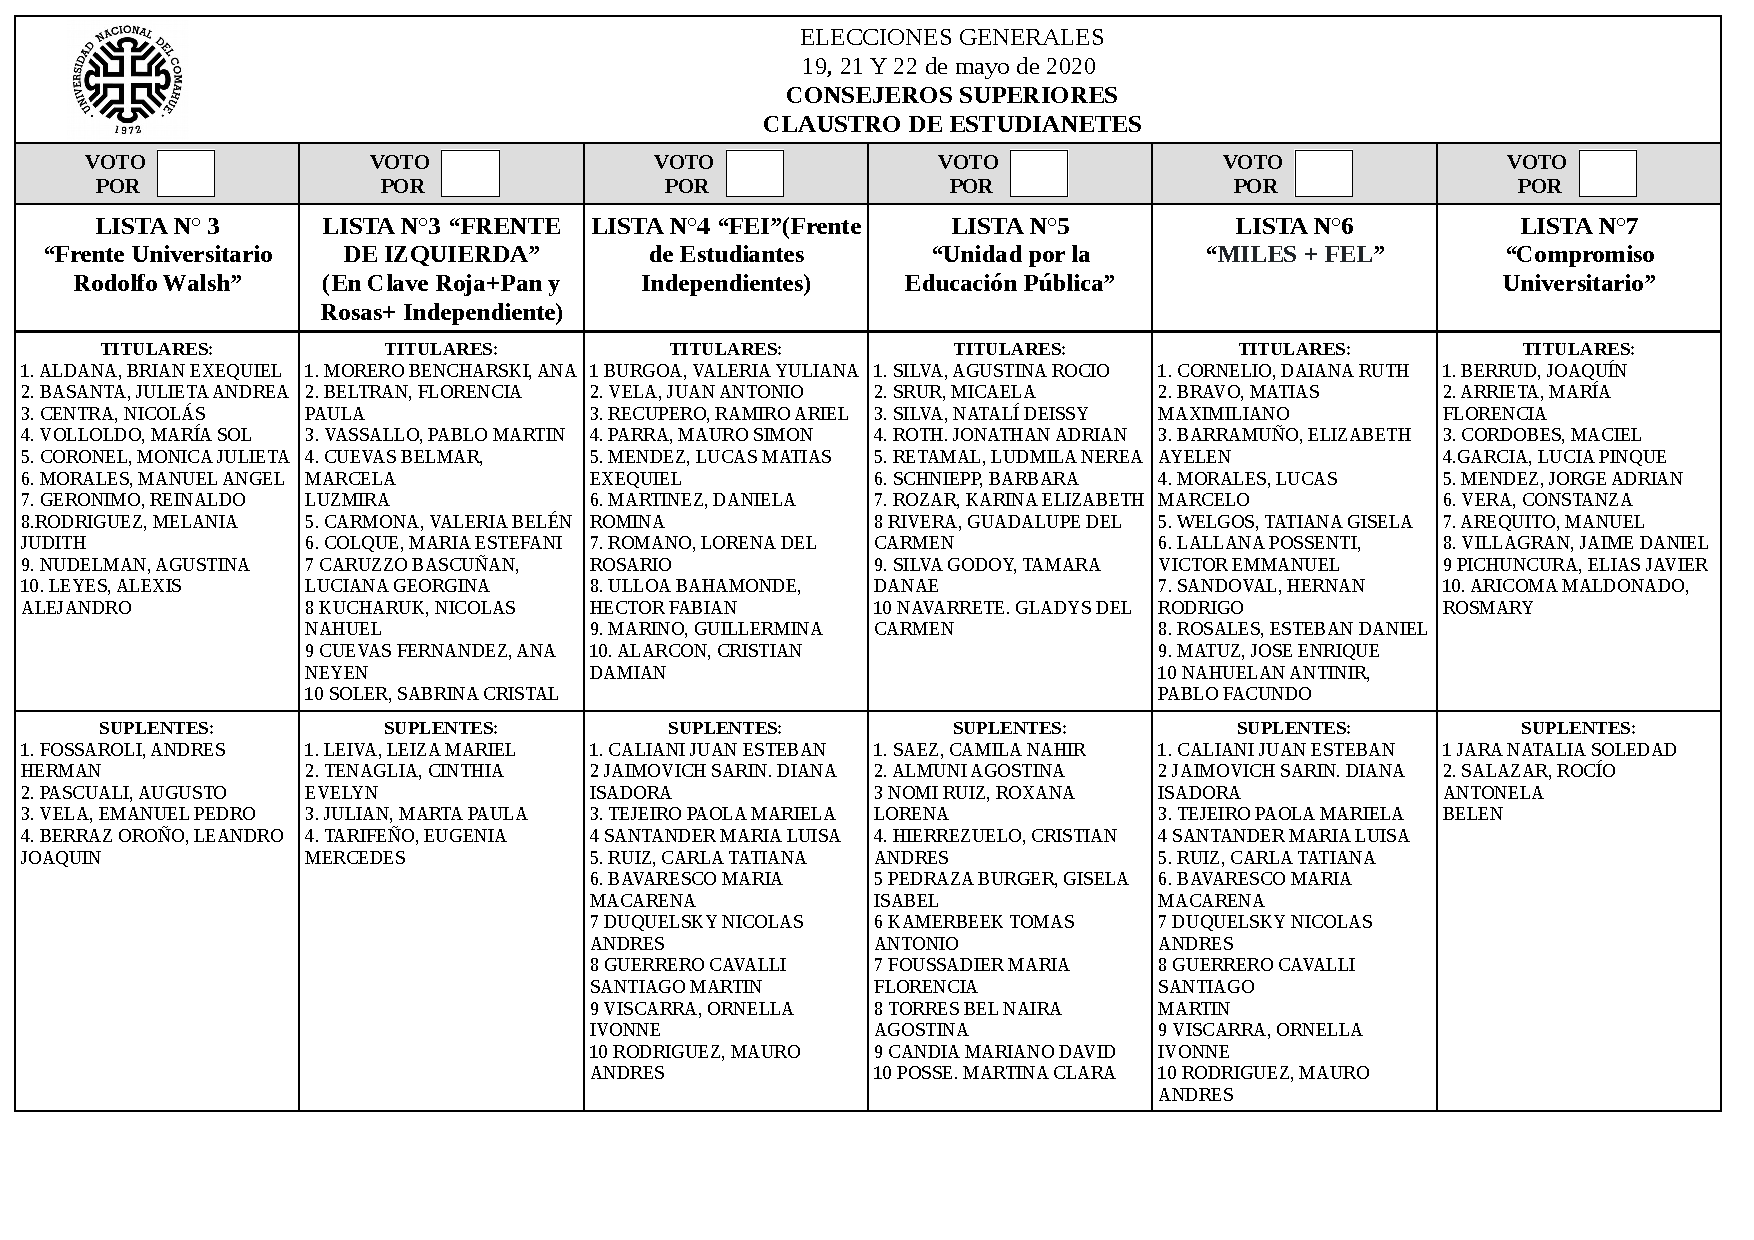
\includepdf[pages=-]{pdf/bue_uncoma.pdf}


\chapter{Anexo III: Documentación Base de Datos Gukena}
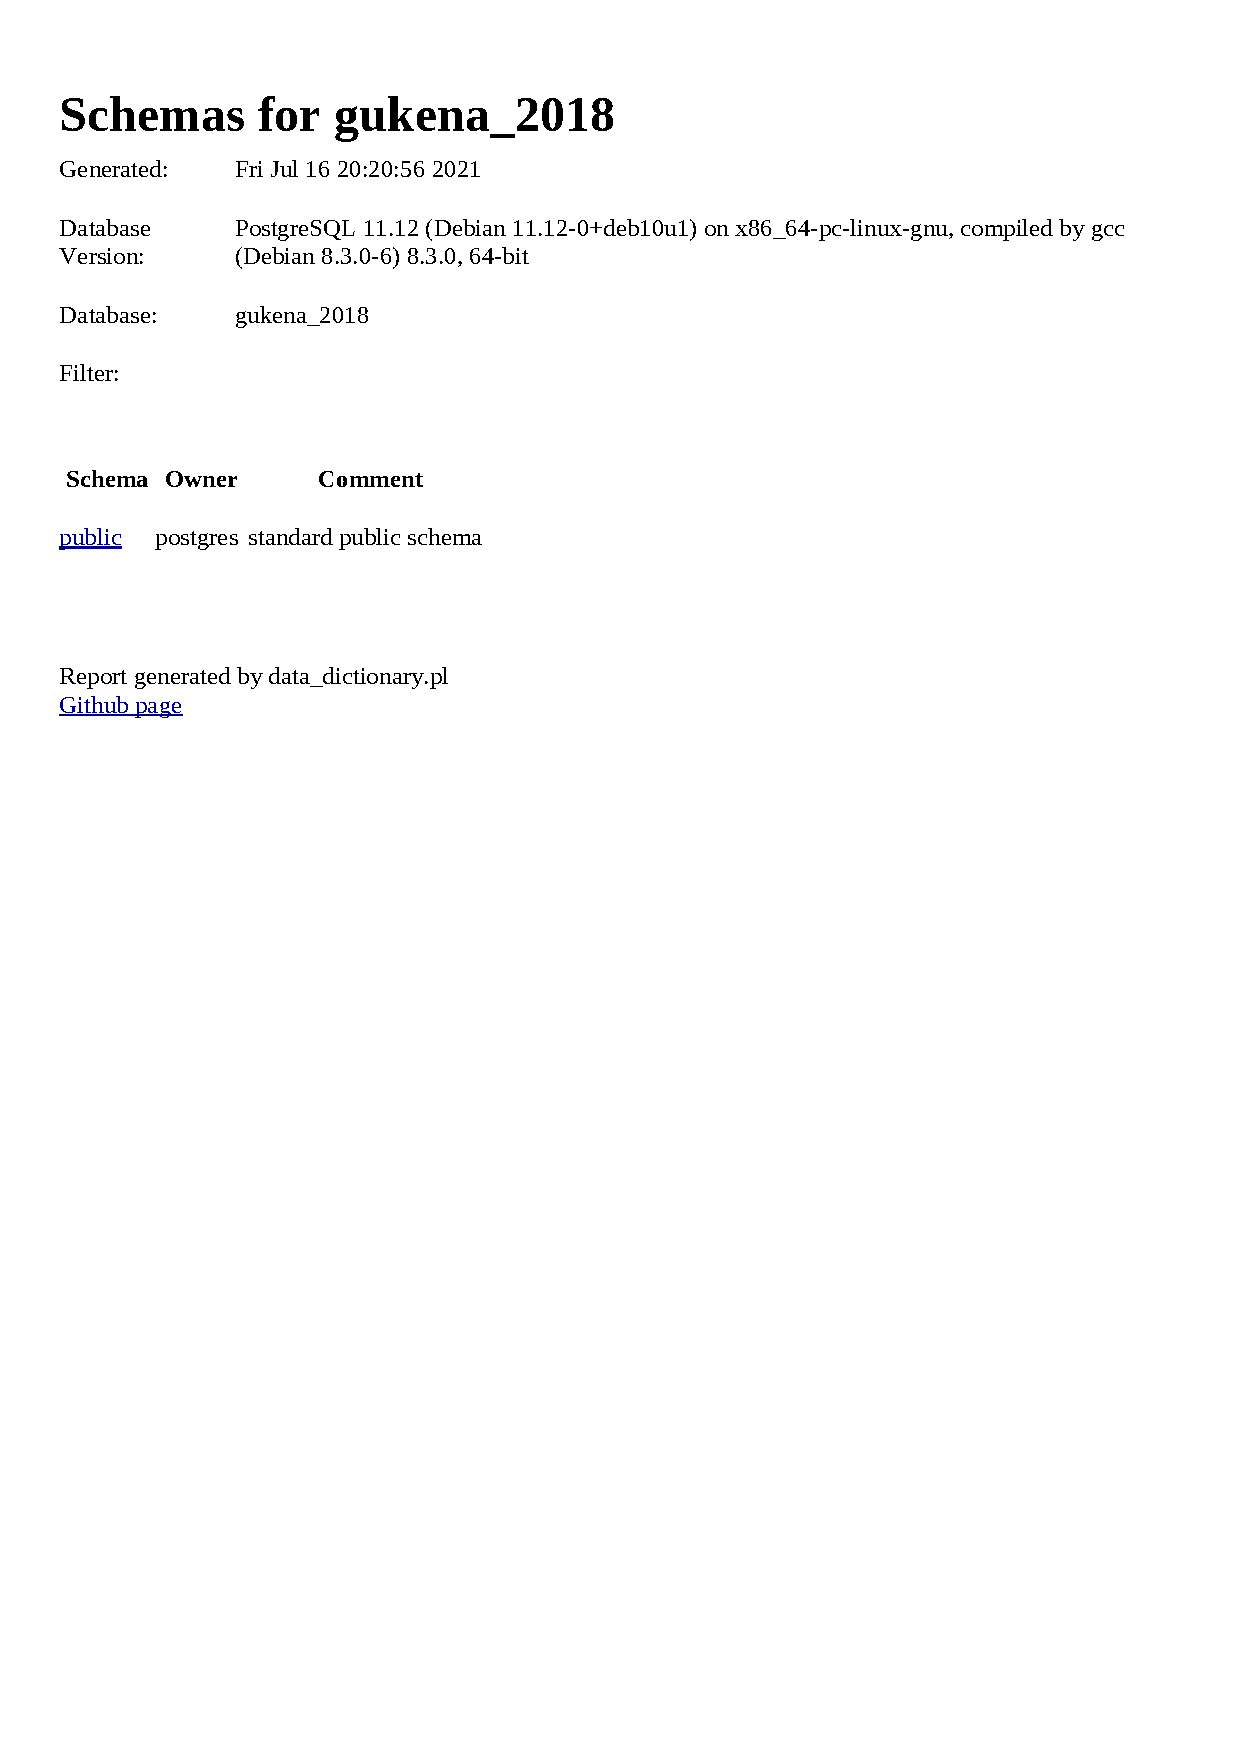
\includepdf[pages=-]{pdf/squema.pdf}
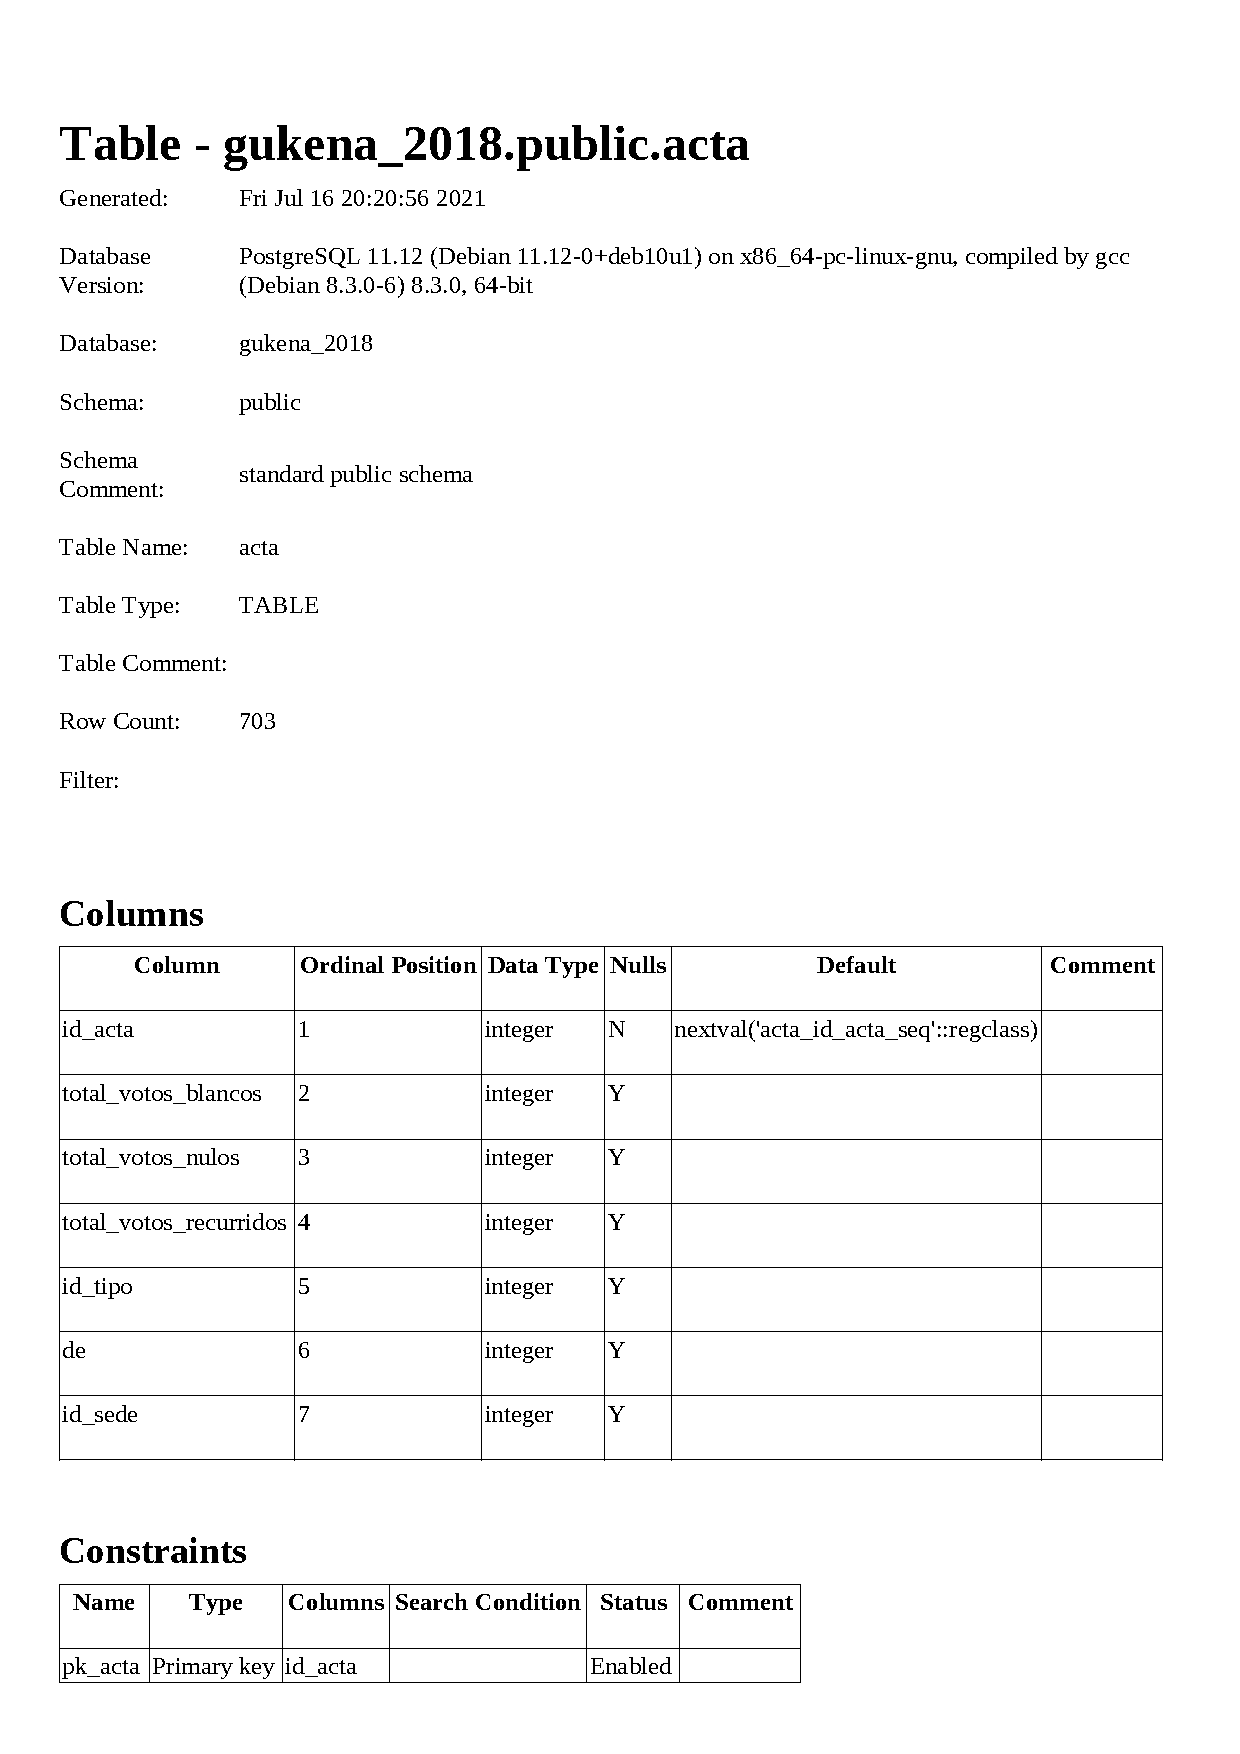
\includepdf[pages=-]{pdf/tables.pdf}
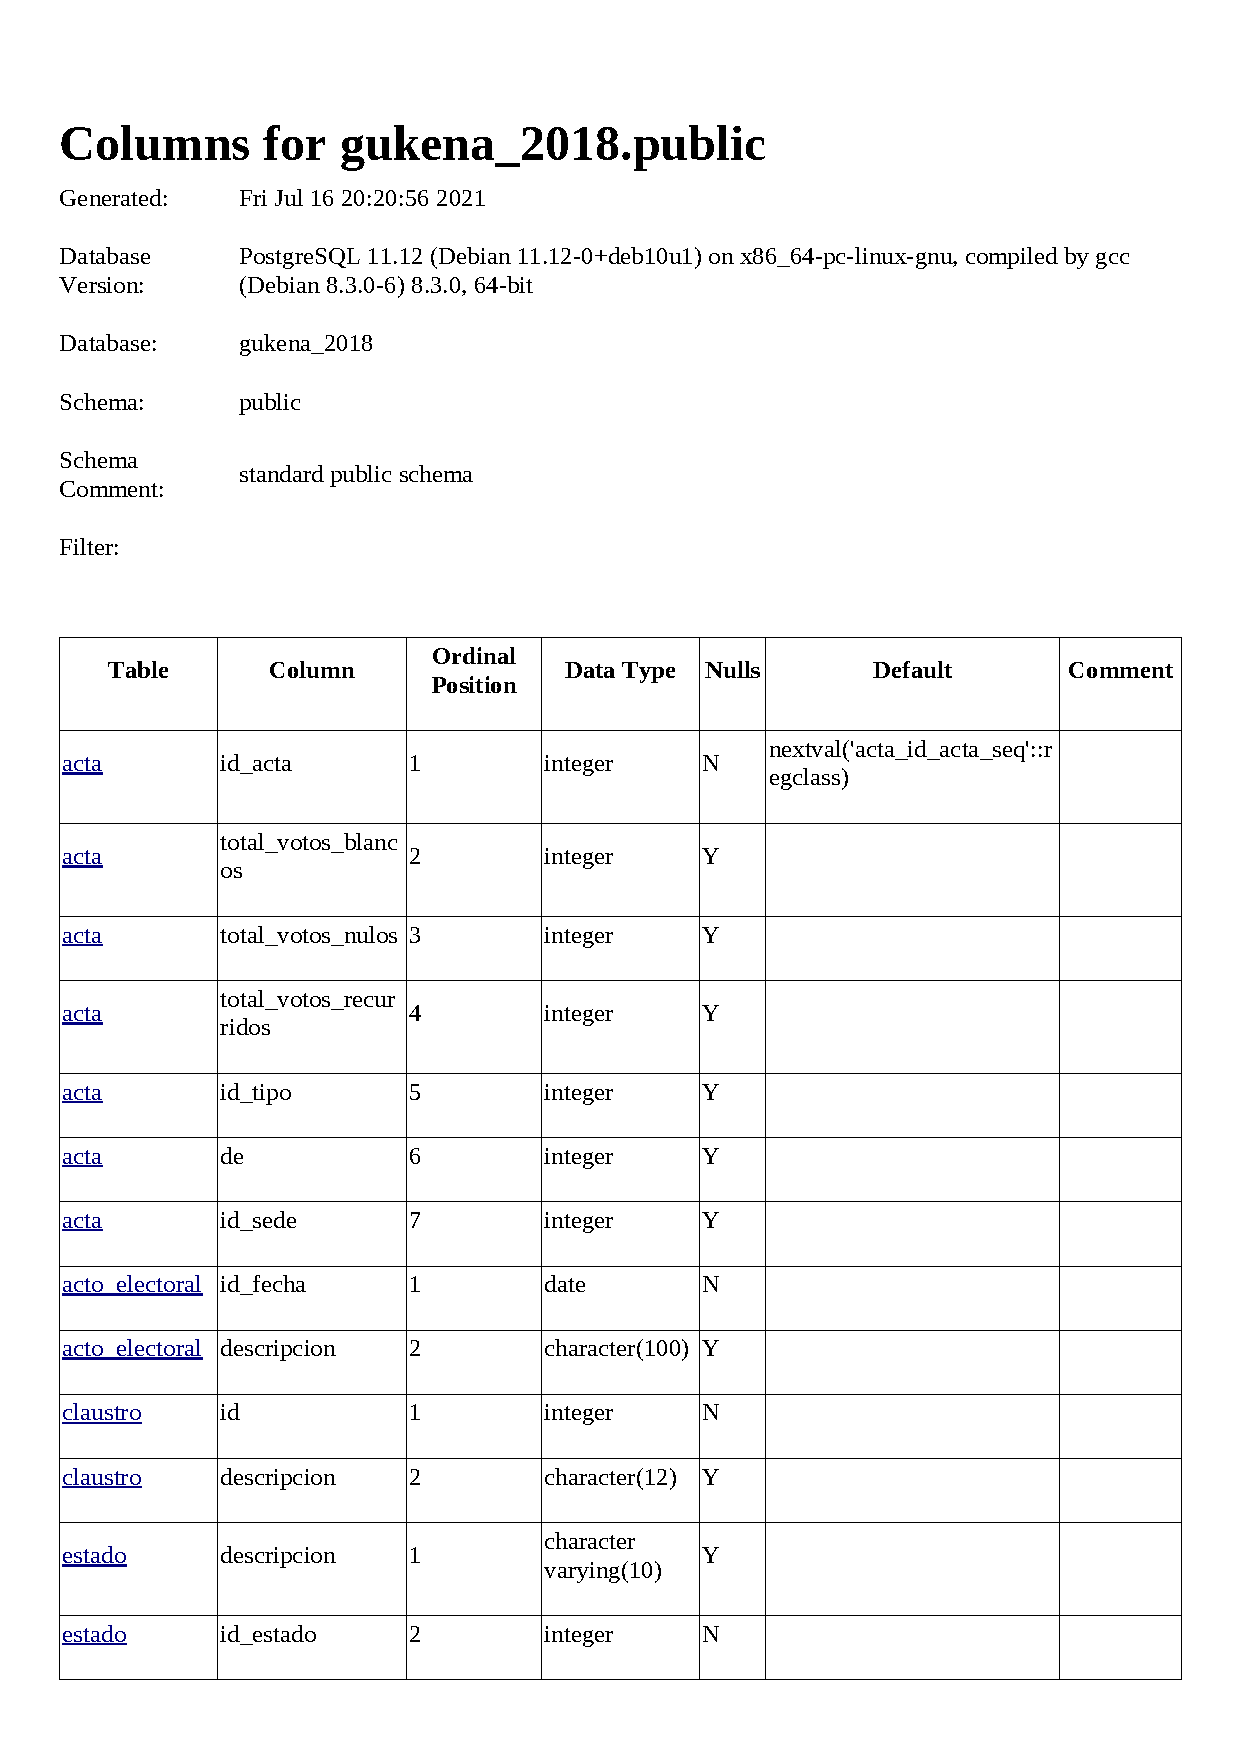
\includepdf[pages=-]{pdf/columns.pdf}
